% Source: Code/FLIR_Python/architecture_diagrams/system_architecture.tex
\documentclass[border=10pt]{standalone}
\usepackage{tikz}
\usepackage{xcolor}
\usetikzlibrary{shapes.geometric, arrows.meta, positioning, fit, backgrounds, calc}

% USC Color Definitions
\definecolor{uscgarnet}{HTML}{73000a}
\definecolor{uscatlantic}{HTML}{466A9F}
\definecolor{usccongaree}{HTML}{1F414D}
\definecolor{uschorseshoe}{HTML}{65780B}
\definecolor{uscrose}{HTML}{CC2E40}
\definecolor{uscsandstorm}{HTML}{FFF2E3}
\definecolor{uscwarmgrey}{HTML}{676156}

\begin{document}

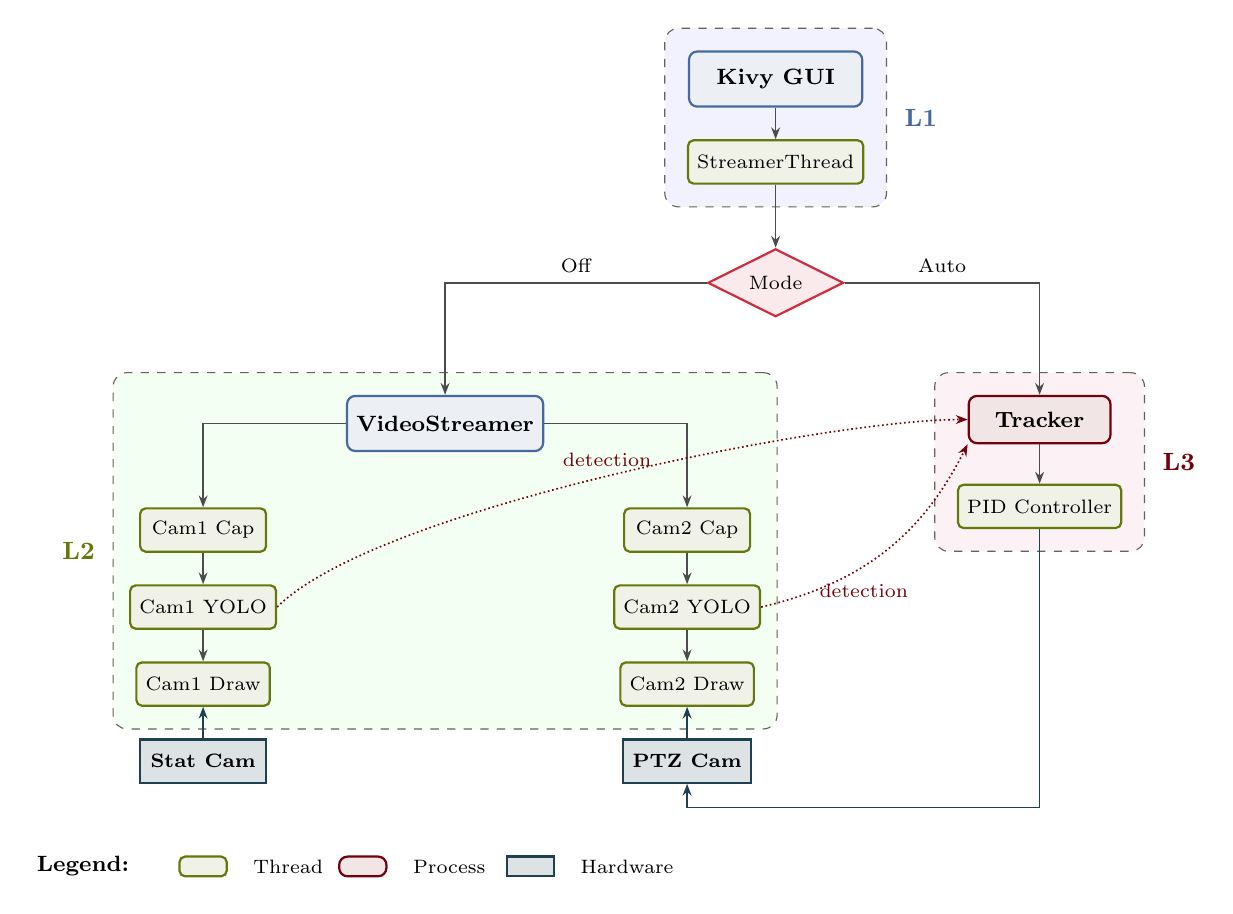
\begin{tikzpicture}[
    % Node styles - slightly smaller (USC Colors)
    app/.style={rectangle, draw=uscatlantic, fill=uscatlantic!10, thick, minimum width=2.2cm, minimum height=0.7cm, align=center, rounded corners=3pt, font=\footnotesize\bfseries},
    thread/.style={rectangle, draw=uschorseshoe, fill=uschorseshoe!10, thick, minimum width=1.6cm, minimum height=0.55cm, align=center, rounded corners=2pt, font=\scriptsize},
    process/.style={rectangle, draw=uscgarnet, fill=uscgarnet!10, thick, minimum width=1.8cm, minimum height=0.6cm, align=center, rounded corners=3pt, font=\footnotesize\bfseries},
    hardware/.style={rectangle, draw=usccongaree, fill=usccongaree!15, thick, minimum width=1.6cm, minimum height=0.55cm, align=center, font=\scriptsize\bfseries},
    decision/.style={diamond, draw=uscrose, fill=uscrose!10, thick, aspect=2, align=center, font=\scriptsize},
    container/.style={draw=uscwarmgrey, dashed, rounded corners=5pt, inner sep=8pt},
    % Arrow styles
    dataarrow/.style={-{Stealth[length=1.5mm]}, semithick, draw=black!70},
    ipc/.style={-{Stealth[length=1.5mm]}, semithick, draw=uscgarnet, densely dotted},
    hwlink/.style={-{Stealth[length=1.5mm]}, semithick, draw=usccongaree},
]

% ============================================================================
% LAYER 1: GUI (Top)
% ============================================================================
\node[app] (gui) {Kivy GUI};
\node[thread, below=0.4cm of gui] (streamer) {StreamerThread};

% Container for L1
\begin{scope}[on background layer]
    \node[container, fill=blue!5, fit=(gui)(streamer)] (l1box) {};
\end{scope}

% L1 label - OUTSIDE the box
\node[right=0.1cm of l1box, font=\small\bfseries\color{uscatlantic}] {L1};

\draw[dataarrow] (gui) -- (streamer);

% ============================================================================
% Mode Switch
% ============================================================================
\node[decision, below=0.8cm of streamer] (mode) {Mode};

\draw[dataarrow] (streamer) -- (mode);

% ============================================================================
% LAYER 2: VideoStreamer - WIDER LAYOUT with hardware directly below
% ============================================================================
\node[app, below left=1.2cm and 2.5cm of mode] (videostreamer) {VideoStreamer};

% Camera 1 Pipeline (far left) - with hardware directly below
\node[thread, below left=0.7cm and 1cm of videostreamer] (cam1cap) {Cam1 Cap};
\node[thread, below=0.4cm of cam1cap] (cam1yolo) {Cam1 YOLO};
\node[thread, below=0.4cm of cam1yolo] (cam1draw) {Cam1 Draw};
\node[hardware, below=0.4cm of cam1draw] (statcam) {Stat Cam};

% Camera 2 Pipeline (right of cam1) - with hardware directly below
\node[thread, below right=0.7cm and 1cm of videostreamer] (cam2cap) {Cam2 Cap};
\node[thread, below=0.4cm of cam2cap] (cam2yolo) {Cam2 YOLO};
\node[thread, below=0.4cm of cam2yolo] (cam2draw) {Cam2 Draw};
\node[hardware, below=0.4cm of cam2draw] (ptzcam) {PTZ Cam};

% Container for L2
\begin{scope}[on background layer]
    \node[container, fill=green!5, fit=(videostreamer)(cam1cap)(cam1draw)(cam2cap)(cam2draw)] (l2box) {};
\end{scope}

% L2 label - OUTSIDE the box on the left
\node[left=0.1cm of l2box, font=\small\bfseries\color{uschorseshoe}] {L2};

% L2 internal connections
\draw[dataarrow] (videostreamer) -| (cam1cap);
\draw[dataarrow] (videostreamer) -| (cam2cap);
\draw[dataarrow] (cam1cap) -- (cam1yolo);
\draw[dataarrow] (cam1yolo) -- (cam1draw);
\draw[dataarrow] (cam2cap) -- (cam2yolo);
\draw[dataarrow] (cam2yolo) -- (cam2draw);

% Mode to VideoStreamer - with Off label above the line
\draw[dataarrow] (mode) -| node[above, font=\scriptsize, pos=0.25] {Off} (videostreamer);

% ============================================================================
% LAYER 3: Tracker Process (Right side)
% ============================================================================
\node[process, below right=1.2cm and 2cm of mode] (tracker) {Tracker};
\node[thread, below=0.5cm of tracker] (pid) {PID Controller};

% Container for L3
\begin{scope}[on background layer]
    \node[container, fill=purple!5, fit=(tracker)(pid)] (l3box) {};
\end{scope}

% L3 label - OUTSIDE the box on the right
\node[right=0.1cm of l3box, font=\small\bfseries\color{uscgarnet}] {L3};

% Mode to Tracker
\draw[dataarrow] (mode) -| node[above, font=\scriptsize, pos=0.25] {Auto} (tracker);

% Internal tracker flow
\draw[dataarrow] (tracker) -- (pid);

% ============================================================================
% Hardware connections - DIRECT VERTICAL (no crossing boxes)
% ============================================================================
\draw[hwlink] (statcam) -- (cam1draw);
\draw[hwlink] (ptzcam) -- (cam2draw);

% PID to PTZ - route around the right side
\draw[hwlink] (pid.south) |- ([yshift=-0.3cm]ptzcam.south) -- (ptzcam.south);

% ============================================================================
% KEY TRACKING FLOW CONNECTIONS - CURVED DOTTED LINES
% ============================================================================

% Cam1 YOLO --"detection"--> Tracker (coarse acquisition)
% Curved line from right side of cam1yolo, going higher between videostreamer and cam2cap
\draw[ipc, out=45, in=180, looseness=0.5] (cam1yolo.east) to node[above, font=\scriptsize, uscgarnet, pos=0.5] {detection} (tracker.west);

% Cam2 YOLO --"detection"--> Tracker (fine tracking)  
\draw[ipc, bend right=25] (cam2yolo.east) to node[below, font=\scriptsize, uscgarnet, pos=0.4, yshift=-0.1cm] {detection} (tracker.south west);

% ============================================================================
% Legend - WELL SPACED with full words visible
% ============================================================================
\node[below left=0.8cm and 0cm of statcam, font=\footnotesize\bfseries] (legend) {Legend:};

\node[thread, right=0.5cm of legend, minimum width=0.6cm, minimum height=0.25cm] (lt) {};
\node[right=0.2cm of lt, font=\scriptsize] {Thread};

\node[process, right=0.6cm of lt, minimum width=0.6cm, minimum height=0.25cm, xshift=0.8cm] (lp) {};
\node[right=0.2cm of lp, font=\scriptsize] {Process};

\node[hardware, right=0.6cm of lp, minimum width=0.6cm, minimum height=0.25cm, xshift=0.9cm] (lh) {};
\node[right=0.2cm of lh, font=\scriptsize] {Hardware};

\end{tikzpicture}

\end{document}
